\documentclass{article}

\usepackage{graphicx}

\begin{document}
	\section*{Lab2 - Filip Jędrzejewski}
	
	\subsection*{Cel zadania}
	
	Celem zadania było zastosowanie metody najmniejszych kwadratów do predykcji, czy 	nowotwór jest złośliwy czy łagodny. Do rozwiązania problemu wykorzystano bibliotekę 		\texttt{pandas}, typ \texttt{DataFrame} oraz dwa zbiory danych: \newline
	- \texttt{breast-cancer-train.dat}\\
	- \texttt{breast-cancer-validate.dat}\\
	Są to zbiory zawierające wartości dziesięciu cech wykrytych nowotworów oraz to czy dany nowotwór był złośliwy czy łagodny.
	
	\subsection*{Histogramy}
	
	Na podstawie powyzszych zbiorów stworzono cztery histogramy roznych kolumn tych danych.
	
	\begin{figure}[h]
    		\centering
  		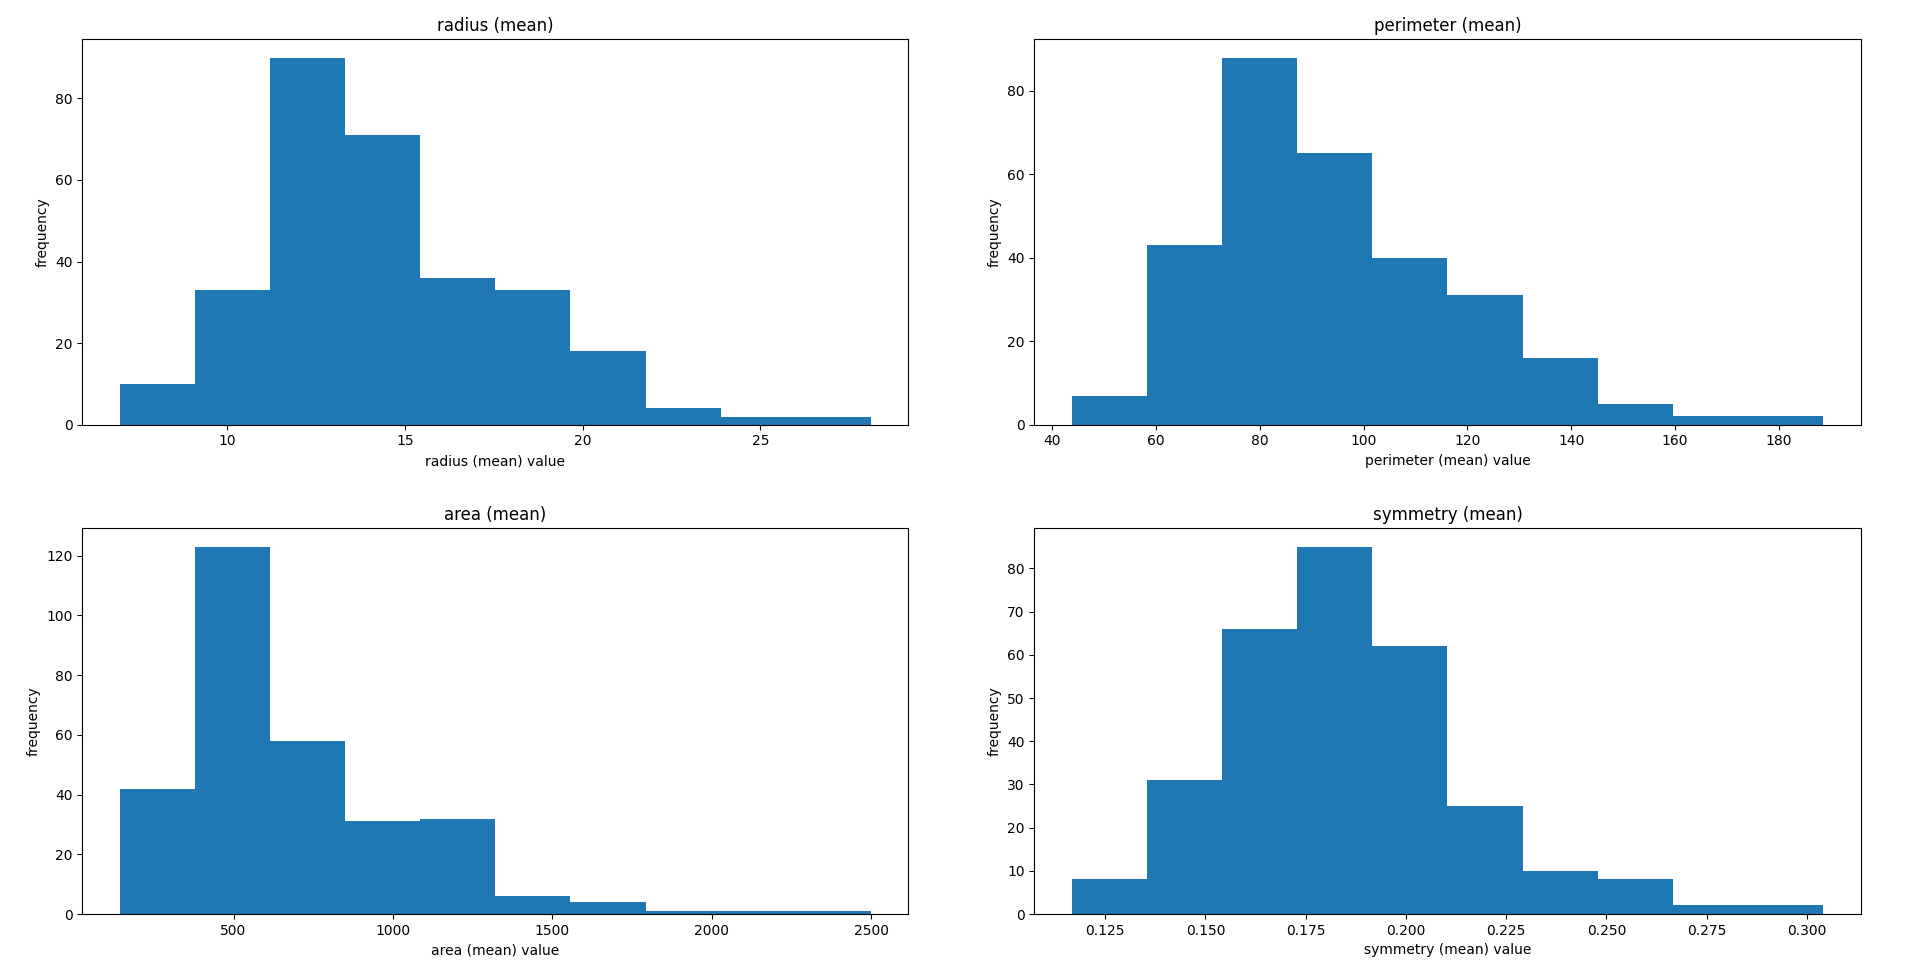
\includegraphics[scale = 0.25]{histograms.png}
	\end{figure}
	
	\subsection*{Przygotowanie danych i wyznaczenie wektorów wag}
	
	W celu predykcji typu nowotworu stworzono reprezentacje macierzową obu zbiorów danych dla liniowej i kwadratowej metody najmniejszych kwadratów (łącznie 4 macierze). Do reprezentacji kwadratowej zostały użyte tylko 4 kolumny: \texttt{radius (mean)}, \texttt{perimeter (mean)}, \texttt{area (mean)}, \texttt{symmetry (mean)}.\\
	W kolejnym kroku utworzono wektory $b$ dla obu zbiorów, których elementy były równe $1$ gdy nowotwór w danym wierszu był złośliwy lub $-1$ w przeciwnym przypadku.\\
	Następnie za pomocą funkcji \texttt{scipy.linalg.lstsq} wyznaczono macierz wag dla kwadratowej i liniowej reprezentacji najmniejszych kwadratów. \\
	
	\subsection*{Współczynniki uwarunkowania}
	
	Za pomocą funkcji \texttt{numpy.linalg.cond} obliczono współczynniki uwarunkowania zarówno dla liniowej, jak i kwadratowej metody najmniejszych kwadratów:
	
	$$cond(A) = 192499.8$$
	$$cond(A_{quad}) = 951673088.7$$
	
	\subsection*{Ocena wyników}
	
	Na końcu sprawdzono jakość otrzymanych wyników. W tym celu wymnożono macierze stworzone ze zbioru \texttt{breast-cancer-validate.dat} z odpowiadającymi im macierzami wag. Wynikami tych działań były wektory $p$ i $p_{quad}$, które zawierały wyniki predykcji. Jeżeli $i$-ty element wektora $p$ był większy od zera, to $i$-ta osoba najpewniej miała nowotwór złośliwy w przeciwnym przypadku ($p_i \leq 0$) osoba miała prawdopodobnie nowotwór łagodny. \\
	Porównano otrzymane wyniki z danymi z wektora $b_{validate}$, który przechowywał prawdziwe wyniki. Na tej podstawie obliczono liczbę wyników fałszywie dodatnich, fałszywie ujemnych, prawdziwie dodatnich i prawdziwie ujemnych. Wyniki zapisano w tabeli:
	
	\begin{center}
		\caption{Wyniki dla reprezentacji liniowej}
		\begin{tabular}{|c|c|c|}
  			\hline 
  			 & osoba zdrowa & osoba chora\\
  			\hline
  			wynik dodatni & 10 & 58 \\
  			\hline
  			wynik ujemny & 190 & 2 \\
  			\hline
		\end{tabular} 
		
	\end{center}
		
		
	
	\begin{center}
		\caption{Wyniki dla reprezentacji kwadratowej}
		\begin{tabular}{|c|c|c|}
  			\hline 
  			 & osoba zdrowa & osoba chora\\
  			\hline
  			wynik dodatni & 15 & 55 \\
  			\hline
  			wynik ujemny & 185 & 5 \\
  			\hline
		\end{tabular} 
		
	\end{center}
	
	\subsection*{Wnioski}
	
	Na podstawie tych tabel oraz wyznaczonych współczynników uwarunkowania możemy zauważyć, że reprezentacja liniowa metody najmniejszych kwadratów jest w tym zadaniu dokładniejsza i lepsza.
	
	
	
	
	
	
	
	
	
	
	
	
	
	
	
	
	
	
	
	
	
	
	
	
	
	
	
	
	
	
	
	
\end{document}